\chapter{Model  for  the study  of  a  cooling elastic-plated  gravity
  current}
\label{chap3}
\minitoc

We present here  a general model, based on  the elastic-plated gravity
current  model developed  in  the  last section,  to  account for  the
cooling of the magmatic intrusion.

\section{Theory}
\label{C3-sec:theory}

\subsection{Formulation}
\label{C3-sec:formulation}

We model an axisymmetric fluid  blister of thickness $h(r,t)$ below an
elastic layer  of constant thickness  $d_c$ and above a  semi infinite
rigid layer \citep{Michaut:2011kg}  (Figure \ref{C3-sketch}) The fluid
is injected  continuously at the base  and center of the  blister at a
rate $Q(t)$  through a  conduit of  diameter $a$.  The hot  fluid is
intruded at temperature $T_i$ and cools through the top and the bottom
by conduction  in the surrounding  medium, whose temperature  $T_s$ is
allowed to increase with time.

\begin{figure}[htbp]
  \begin{center}
    \graphicspath{ {/Users/thorey/Documents/These/Manuscript/Figure/Chapter3/} }
    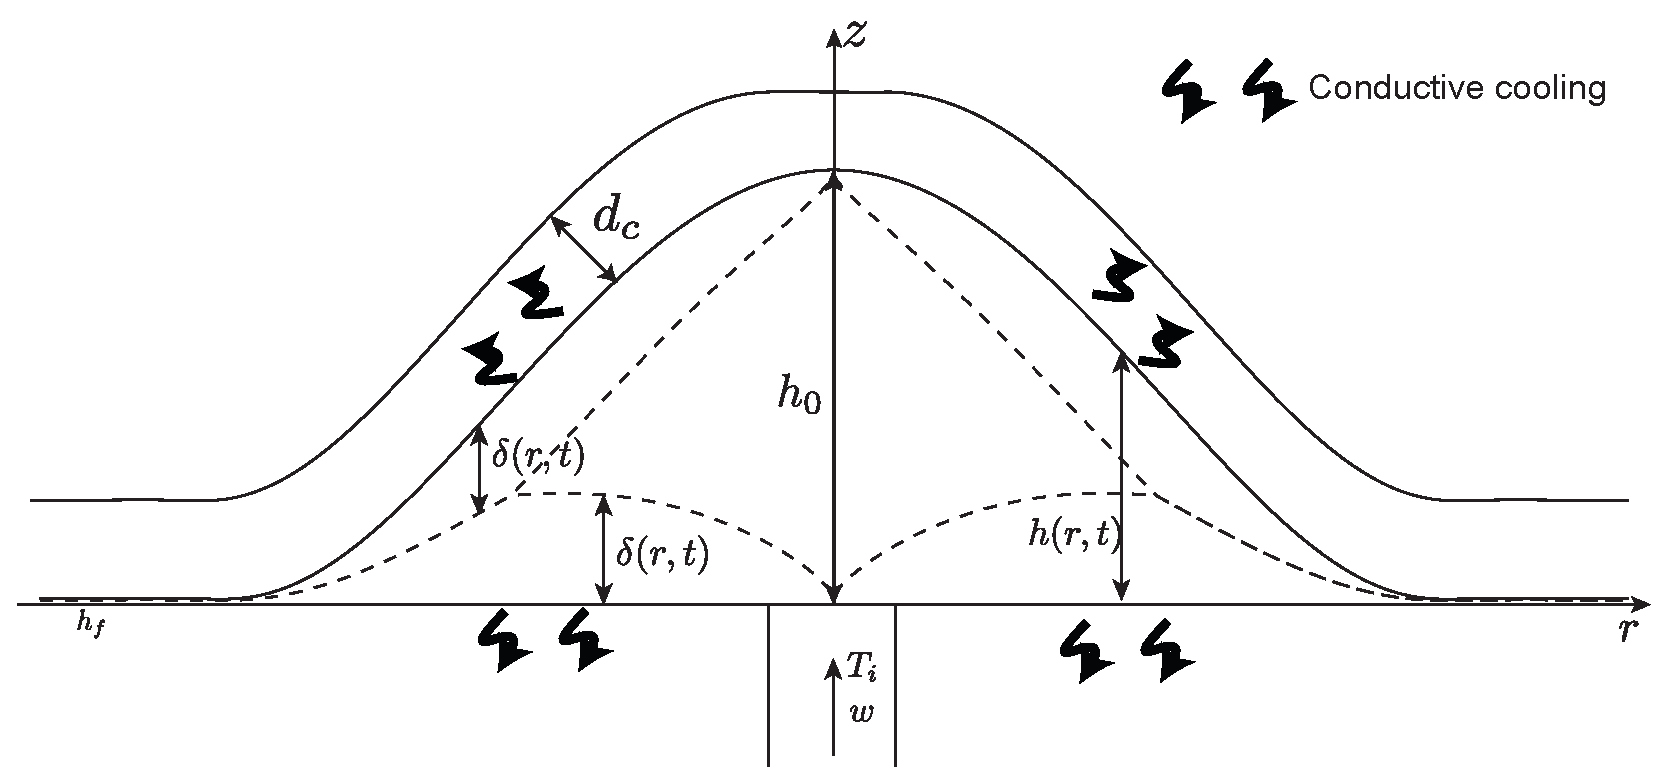
\includegraphics[scale=0.40]{C3-sketch.pdf}
    \caption{Model geometry and parameters.}
    \label{C3-sketch}
  \end{center}
\end{figure}

As  it  cools,  the  viscosity  of the  fluid  increases  following  a
prescribed  rheology   $\eta(T)$  bounded  between  two   values:  the
viscosity of the  hottest fluid $\eta_h$ at temperature  $T_i$ and the
viscosity of the coldest fluid $\eta_c$ at temperature $T_0$.

\subsection{Thickness equation}

For  a cooling  elastic-plated  gravity current,  the velocity  fields
depends   on   the   viscosity,    which   itself   depends   on   the
temperature. Without knowledge on the  form of the rheology $\eta(T)$,
integrating twice  (\ref{C2_V1}) using no-slip boundary  conditions at
the top and the bottom now gives
\begin{equation}
  u(r,z,t) = \frac{\partial P}{\partial r}\left(I(z)-I(h)\frac{z}{h}\right)
\end{equation}
with
\begin{equation}
  I(z) = \int_0^z\frac{z^*}{\eta(T)}dz^*
\end{equation}
where the driving pressure $P(r,z,t)$ is given by (\ref{C2-pression}).
However, instead of plugging in  this expression in (\ref{C2-Mass}) as
in  section   \ref{C2-sec:Governing  equation},  we   develop  another
approach  which ends  in  a  nicer form  for  the thickness  evolution
equation. We first remark that
\begin{equation}
  \int_0^h u dz = -\int_0^h\frac{\partial u}{\partial z}zdz
\end{equation}
and therefore, the statement  of mass conservation (\ref{C2-Mass}) can
be written
\begin{eqnarray}
  \frac{\partial         h}{\partial        t} -\frac{1}{r}
  \frac{\partial}{\partial
  r} \left( r\int_0^h\frac{\partial u}{\partial z}zdz\right) = w_i.
  \label{C3-Mass}
\end{eqnarray}



Integrating  once (\ref{C2_V1})  using  the symmetry  of the  velocity
$u(r,z,t)$ around $h/2$ gives
\begin{equation}
  \frac{\partial u}{\partial z} = \frac{1}{\eta}\frac{\partial P}{\partial r}\left(z-\frac{h}{2}\right)
\end{equation}
which we can now plug in into 
\begin{eqnarray}
  \frac{\partial         h}{\partial        t} -\frac{1}{r}
  \frac{\partial}{\partial
  r} \left( r\int_0^h\frac{\partial u}{\partial z}zdz\right) = w_i.
  \label{C3-Mass}
\end{eqnarray}


The vertical temperature structure described in the following posses a
symmetry around $h/2$ and so the viscosity and the velocity.



As  in  section  \ref{C2-sec:Governing  equation},  we  plug  in  this
expression for  the velocity in  a global  a global statement  of mass
conservation gives and the equation for the thickness evolution reads
\begin{eqnarray}
  \frac{\partial         h}{\partial        t} +\frac{1}{r}
  \frac{\partial}{\partial
  r} \left( r\int_0^hudz\right) = w_i
  \label{C2-Mass}
\end{eqnarray}

\subsection{Heat transport equation}

\subsubsection{Local energy conservation}\\

In the laminar regime and in axisymmetrical coordinates ($r$,$z$), the
local energy  conservation equation within the  lubrication assumption
is written as
\begin{eqnarray}
  \frac{D}{D t}\left(\rho_m C_{p,m} T+\rho_mL(1-\phi)\right)&=& k_m  \frac{\partial^2
                                                                T}{\partial
                                                                z^2}
\label{C3-EnergyCons}
\end{eqnarray}

where  $T(r,z,t)$  is  the  fluid temperature,  $\phi(r,z,t)$  is  the
crystal fraction  in the melt  and $\rho_m$, $k_m$, $C_{p,m}$  and $L$
are the density,  thermal conductivity, specific heat  and latent heat
of the  fluid.  In this model,  the crystals are considered  only as a
source/sink of energy  as they melt/form during  the flow emplacement.
In particular, they share the same properties that the fluid itself.

Following a common approximation, we  assume that the crystal fraction
is a linear function of temperature over the melting interval
\begin{equation}
  \phi = \frac{T_L-T}{T_L-T_s}
  \label{C3-meltfraction}
\end{equation}
where $T_S$ and $T_L$ are the solidus and liquidus temperatures of the
magma  \citep{Hort:1997hk,Michaut:2006di}.   With this  approximation,
the local energy equation (\ref{C3-EnergyCons}) resumes to
\begin{eqnarray}
  \frac{\partial T}{\partial t}+ u\frac{\partial T}{\partial r}
  + w\frac{\partial T}{\partial z}  &=& \frac{ \kappa_m}{1+St^{-1}}  \frac{\partial^2
                                        T}{\partial               z^2}
                                        \label{C3-EnergyCons2}
\end{eqnarray}
where  $u(r,z,t)$ and  $w(r,z,t)$ are  the radial  and vertical  fluid
velocities,  $St  =\left(C_{p,m}(T_L-T_S)\right)/L$   is  the  Stephan
number   and    $\kappa_m$   is   the   fluid    thermal   diffusivity
$\kappa_m = k_m/\rho_m  C_{p,m}$.  Following \citet{BALMFORTH:2004fm},
we use an integral balance method to solve the heat transport equation
(\ref{C3-EnergyCons2}).   This theory  is based  on the  integral-balance
method of heat-transfer theory of \citet{Goodman:1958ue}, in which the
vertical structure of the temperature  field is represented by a known
function of depth that approximates the expected solution.

\subsubsection{Integral   balance   solution   for   the   temperature
  $T(r,z,t)$}

We model  the cooling of the  fluid blister through the  growth of two
thermal  boundary layers:  one growing  downward  from the  top and  a
second  growing upward  from  the base.   As  we consider  homogeneous
thermal properties for  the surrounding rocks, we assume  that the two
thermal boundary layers grow symmetrically and have the same thickness
$\delta(r,t)$.   In agreement,  the integral-balance  approximation we
use for the vertical temperature profile $T(r,z,t)$ is
\begin{equation}
  T=
  \begin{cases}
    T_b - (T_b-T_s)(1-\frac{z}{\delta})^2 & 0 \le z\le \delta \\
    T_b & \delta \le z\le h-\delta \\
    T_b - (T_b-T_s)(1-\frac{h-z}{\delta})^2 & h-\delta \le z\le h\\
  \end{cases}
  \label{C3-Temperature}
\end{equation}
where $T_b(r,t)$  is the  temperature at  the center  of the  flow and
$T_s(r,t)$ the temperature  at the contact with  the surrounding rocks
(Figure   \ref{Figure2-1}).    The   integral  balance   solution   in
(\ref{C3-Temperature}) assumes  a symmetry around $z=h/2$  and a decrease
of the  temperature in  the two  thermal boundary  layers down  to the
surrounding  rock  temperature   $T_s$  \citep{BALMFORTH:2004fm}.   In
addition,  it  assumes a  uniform  temperature  $T_b$ in  between  the
thermal  boundary  layers.   Then,  as  the fluid  is  injected  at  a
temperature  $T_i$,   we  have  $T_b(r,t)  =T_i$   when  $\delta<h/2$.
However,   if  the   two   thermal  boundary   layers  connect,   then
$\delta = h/2$ and $T_b$ decreases such that $T_b\le T_i$.

\subsubsection{Integral balance equation}
\label{C3-sec:integr-balance-equat}

We   begin    by   integrating    the   local    energy   conservation
(\ref{C3-EnergyCons2})  over  the  two   thermal  boundary  layers.   The
integration over the  bottom thermal layer, i.e. from  the base, $z=0$
to a level $z = \delta$ gives
\begin{eqnarray}
  &&\frac{\partial}{\partial t}\left( \delta( \bar{T}-T_b)\right)+\frac{1}{r}\frac{\partial}{\partial r} \left( r\delta(\overline{uT}-\bar{u}T_b)\right) + \delta\left( \frac{\partial T_b}{\partial t}+ \overline{u}\frac{\partial T_b}{\partial r}\right)\nonumber\\
  &=&-\frac{\kappa_m}{1+St^{-1}}\left. \frac{\partial T}{\partial z}\right|_{z=0}+w_{i}(T_{i}-T_b)
      \label{C3-Local1}
\end{eqnarray}
where the  bar indicate the  vertical average over the  bottom thermal
boundary layer
\begin{equation}
  \overline{f} = \frac{1}{\delta}\int_0^{\delta}f dz\nonumber,
\end{equation}
$T_b(r,t)$  is  the temperature  at  $z=\delta$,  $w_{i}(r)$ is  the
vertical  injection velocity  and  we  have used  the  nullity of  the
thermal gradient at $z=\delta$ and the local mass conservation
\begin{equation}
  \frac{1}{r}\frac{\partial ru}{\partial r} +\frac{\partial w}{\partial z}=0.
  \label{C3-MassConservation}
\end{equation}
The  integration over  the top  thermal layer,  i.e., from  the level,
$z=h-\delta$ to the top $z=h$ gives:
\begin{eqnarray}
  &&\frac{\partial}{\partial t}\left( \delta( \bar{T}-T_b)\right)+\frac{1}{r}\frac{\partial}{\partial r} \left( r\delta(\overline{uT}-\bar{u}T_b)\right) + \delta\left(\frac{\partial T_b}{\partial t}+ \overline{u}\frac{\partial T_b}{\partial r}\right)\nonumber\\
  &=&\frac{\kappa_m}{1+St^{-1}}\left. \frac{\partial T}{\partial z}\right|_{z=h}.
      \label{C3-Local2}
\end{eqnarray}
where,    in    addition    to    the    local    mass    conservation
(\ref{C3-MassConservation})  and   the  fact  the  thermal   gradient  at
$z=h-\delta$ is  equal to  zero, we have  used the  kinematic boundary
condition in $z=h(r,t)$
\begin{equation}
  \frac{\partial h}{\partial t} +u\frac{\partial h}{\partial
    r} = w
\end{equation}
The heat balance equation can then be written by adding (\ref{C3-Local1})
and (\ref{C3-Local2}) and introducing (\ref{C3-Temperature})
\begin{eqnarray}
  &&\frac{\partial}{\partial t}\left( \delta( \bar{T}-T_b)\right)+\frac{1}{r}\frac{\partial}{\partial r} \left( r\delta(\overline{uT}-\bar{u}T_b)\right) + \delta\left( \frac{\partial T_b}{\partial t}+ \overline{u}\frac{\partial T_b}{\partial r}\right)\nonumber\\
  &=&\frac{\kappa_m}{2(1+St^{-1})}\left(\left. \frac{\partial T}{\partial z}\right|_{z=h}-\left. \frac{\partial T}{\partial z}\right|_{z=0}\right)+\frac{w_{i}}{2}(T_{i}-T_b)
      \label{C3-LocalHeat3}
\end{eqnarray}

\subsubsection{Thermal boundary conditions}
\label{C3-sec:thermal-boundary-condition}

At  the  contact with  the  surrounding  rock,  the  heat is  lost  by
conduction:
\begin{equation}
  k_m\left.\frac{\partial                                    T}{\partial
      z}\right|_{z=0}=k_r\left.\frac{\partial              T_r}{\partial
      z}\right|_{z=0}
  \label{C3-Flux1}
\end{equation}
\begin{equation}
  k_m\left.\frac{\partial                                  T}{\partial
      z}\right|_{z=h}=k_r\left.\frac{\partial            T_r}{\partial
      z}\right|_{z=h}
  \label{C3-Flux2}
\end{equation}

where  $T_r(r,z)$  is  the  temperature  in  the  surrounding  medium.
Assuming  a  semi  infinite  layer  for  the  rigid  layer  below  the
intrusion, \citet{Carslaw:1959wf}  show that the temperature  $T_r$ in
the surrounding rocks can be approximated to a first order by
\begin{equation}
  T_r(r,z,t)-T_0=(T_{s}-T_0)\operatorname{erfc}{\left(\frac{-z}{2\sqrt{\kappa_r t}}\right)}.
  \label{eq22}
\end{equation}
The  thickness of  the upper  layer is  equal to  the intrusion  depth
$d_c$. However,  we assume that the  depth $d_c$ is large  compared to
the characteristic  length scale for  conduction $L_c$ and we  use the
same approximation to derive $T_r$ above the intrusion
\begin{equation}
  T_r(r,z,t)-T_0=(T_{s}-T_0)\operatorname{erfc}{\left(\frac{z-h}{2\sqrt{\kappa_r t}}\right)}.
  \label{eq11}
\end{equation}

Therefore,  the  two  thermal boundary  conditions  (\ref{C3-Flux1})  and
(\ref{C3-Flux2}) become:

\begin{equation}
  k_m\left.\frac{\partial                                    T}{\partial
      z}\right|_{z=0}= k_r
  \frac{T_{s}-T_{0}}{\sqrt{\pi \kappa_r t}}
  \label{C3-Flux_1}
\end{equation}
\begin{equation}
  k_m\left.\frac{\partial                                    T}{\partial
      z}\right|_{z=h}= -k_r
  \frac{T_{s}-T_{0}}{\sqrt{\pi \kappa_r t}}
  \label{C3-Flux_2}
\end{equation}


\subsection{Dimensionless equations}
\label{C3-sec:dimens-equat}

The equation for the thickness  evolution have been derived in section
\ref{C2-sec:model} and reads
\begin{equation}
  \frac{\partial h}{\partial t} = \frac{1}{r}
  \frac{\partial}{\partial r} \left( r\left(\rho_m g \frac{\partial h}{\partial      r}+D\frac{\partial}{\partial      r}\left(\nabla^4h\right)\right)I\right)
  + w_i.
  \label{C2-EqConservation}
\end{equation}
where
\begin{equation}
  I = \int_0^h\frac{1}{\eta(T)}\left(z-\frac{h}{2}\right)z dz
  \label{C2-Integral}
\end{equation}
This   equation  is   then  coupled   to  the   heat-balance  equation
(\ref{C3-LocalHeat3})  through  the  viscosity  $\eta(T)$.   We  first
rewrite      the      different       temperatures      such      that
$T=T_0+\left(T_i-T_0)\theta$ where  $\theta(r,z,t)$ is  the equivalent
  dimensionless  temperature.   In  term  of  $\theta$,  the  integral
  balance approximation (\ref{C3-Temperature}) rewrites
  \begin{equation}
    \theta(z)=
    \begin{cases}
      \Theta_b -\left(\Theta_b-\Theta_s\right)(1-\frac{z}{\delta})^2& 0 \le z\le \delta \\
      \Theta_b & \delta \le z\le h-\delta \\
      \Theta_b -\left(\Theta_b-\Theta_s\right)(1-\frac{h-z}{\delta})^2
      & h-\delta \le z\le h
    \end{cases}
    \label{Temperature2}
  \end{equation}
  where            $\Theta_b=\frac{T_b-T_0}{T_{i}-T_0}$            and
  $\Theta_s        =       \frac{T_s-T_0}{T_i-T_0}$.         Equations
  (\ref{C3-LocalHeat3})  and  (\ref{C3-Mass})  are  nondimensionalized
  using the same horizontal scale $\Lambda$, vertical height scale $H$
  and time  scale $\tau$ used is  section \ref{C2-sec:dimens-equat} as
  well        as       a        horizontal       velocity        scale
  $U=\Lambda/\tau=\left(\rho_m          g          H^3\right)/\left(12
    \eta_h\Lambda\right)$ to give
  \begin{eqnarray}
  \frac{\partial h}{\partial t}& =& \frac{1}{r}
  \frac{\partial}{\partial r} \left( r\left(\rho_m g \frac{\partial h}{\partial      r}+D\frac{\partial}{\partial      r}\left(\nabla^4h\right)\right)I\right)
  + w_i\label{EqFinal1}\\
    \frac{\partial}{\partial
    t}\left( \delta( \bar{\theta}-\Theta_b)\right)&=&-\frac{1}{r}\frac{\partial}{\partial
                                                      r}  \left(   r\delta(\overline{u\theta}-\bar{u}\Theta_b)\right)  -
                                                      \delta\left(      \frac{\partial       \Theta_b}{\partial      t}+
                                                      \overline{u}\frac{\partial     \Theta_b}{\partial    r}\right)\nonumber\\
                                 &-&
                                     2Pe^{-1}St_m\frac{\left(\Theta_b-\Theta_s\right)}{\delta}+\frac{w_{i}}{2}(1-\Theta_b)\label{HeatDimensionLess}\\
    u(r,z,t)&   =&   12\left(\rho_m   g   \frac{\partial   h}{\partial
                 r}+D\frac{\partial}{\partial
                   r}\left(\nabla^4h\right)\right)            \int_0^z
                   \frac{1}{\eta(\theta,\nu)}
                   \left(z-\frac{h}{2}\right)dz\label{C3-Veloc}\\
    w_{i}&=&
             \frac{32}{\gamma^{2}}\left(\frac{1}{4}-\frac{r^{2}}{\gamma^{2}}\right)\left(1-\frac{h_0}{\sigma}\right)\hspace{.2cm}
             \text{if} \hspace{.2cm} r < \gamma/2
  \end{eqnarray}
  where $\eta(\theta,\nu)$ is the dimensionless rheology $\eta/\eta_h$
  which  depends on  the  dimensionless temperature  $\theta$ and  the
  dimensionless  number  $\nu$.   In addition,  the  thermal  boundary
  conditions (\ref{C3-Flux_1}) and (\ref{C3-Flux_2}) resume to
  \begin{equation}
    2\frac{\Theta_b-\Theta_s}{\delta}               =               \Omega
    Pe^{1/2}\frac{\Theta_s}{\sqrt{\pi t}}.
    \label{C3-Boundary-Condi}
  \end{equation}
  $\gamma$, $\sigma$,  $Pe$, $St_m$,  $\nu$ and  $\Omega$ are  the six
  dimensionless numbers that control the dynamics of the flow
  \begin{eqnarray}
    \gamma&=&\frac{a}{\Lambda} \label{gamma}\\
    \sigma &=& \frac{\Delta P}{\rho_m g h_0} \label{sigma}\\
    Pe&=& \frac{H^2}{\kappa_m \tau}\label{Pe}\\
    St_m &=& \frac{C_{p,m}\left(T_L-T_S\right)}{C_{p,m}\left(T_L-T_S\right)+L} \label{St}\\
    \nu&=& \frac{\eta_h}{\eta_c}\label{nu}\\
    \Omega&=&\frac{k_r}{k_m}\left(\frac{\kappa_m}{\kappa_r}\right)^{1/2}\label{omega}
  \end{eqnarray}
  $\gamma$ is the dimensionless radius  of the conduit and $\sigma$ is
  the normalized  pressure head which  have been discussed  in section
  \ref{C2-sec:model}.   $Pe$ is  the  Peclet number,  it compares  the
  vertical  diffusion  of heat  to  the  horizontal advection  in  the
  intrusion interior. $St_m$  is a modified Stephan number,  it is the
  ratio of  sensible heat  between solidus and  liquidus to  the total
  energy of  the fluid at liquidus  temperature and tends to  one when
  the  crystallization is  neglected. $\nu$  is the  maximum viscosity
  contrast, i.e.  the ratio between the hottest and coldest viscosity.
  $\Omega$ is  the ratio between  heat conduction at the  contact with
  the encasing rocks and heat diffusion within the fluid.

  \subsection{Further simplifications}
  \label{C3-sec:furth-simpl}

  \textbf{Heat balance equation} \vspace{.5cm}

  The heat balance equations (\ref{HeatDimensionLess}) can reduce to
  \begin{eqnarray}
    \frac{\partial}{\partial
    t}\left( \delta( \bar{\theta}-1)\right)+\frac{1}{r}\frac{\partial}{\partial
    r}
    \left( r\delta(\overline{u\theta}-\bar{u})\right)&=&- 2Pe^{-1}St_m\frac{\left(\Theta_b-\Theta_s\right)}{\delta} 
                                                         \label{HeatD_a}
  \end{eqnarray}

  Indeed, if the thermal boundary layers exist, $\Theta_b=1$, $\delta$
  is    the     variable    and    the    heat     balance    equation
  (\ref{HeatDimensionLess}) reduces  to the  equation (\ref{HeatD_a}).
  In contrast, if the thermal  boundary layers merge, $\delta=h/2$ and
  the variable is $\Theta_b$. In this case, the heat balance equations
  (\ref{HeatDimensionLess}) reduces to:
  \begin{eqnarray}
    \frac{\partial h\bar{\theta}}{\partial t}+\frac{1}{r}\frac{\partial}{\partial
    r} \left( rh\overline{u\theta}\right)-\Theta_b\left(\frac{\partial h}{\partial t}+\frac{1}{r}\frac{\partial}{\partial
    r} \left( rh\bar{u}\right)\right)&=& - 8St_mPe^{-1}\frac{\left(\Theta_b-\Theta_s\right)}{h}+w_{i}(1-\Theta_b)\nonumber
  \end{eqnarray}
  which we can rewrite using (\ref{EqFinal1}) as
  \begin{equation}
    \frac{\partial h\bar{\theta}}{\partial t}+\frac{1}{r}\frac{\partial}{\partial
      r} \left( rh\overline{u\theta}\right) &=& w_i
    - 8St_mPe^{-1}\frac{\left(\Theta_b-\Theta_s\right)}{h}\nonumber\\
  \end{equation}
  which  also  corresponds  to   (\ref{HeatD_a})  in  the  case  where
  $\delta=h/2$.

  \vspace{.5cm} \textbf{Average quantity} \vspace{.5cm}

  Instead   of    injecting   the   expression   for    the   velocity
  (\ref{C3-Veloc}) into the integral appearing in (\ref{EqFinal1}), we
  first integrate by part to get
\begin{eqnarray}
\int_0^h      udz&=&   [    uz   ]_{0}^{\delta}    -\int_0^h
                                                                           z\frac{\partial
                     u}{\partial z} dz \\
&=&-12\frac{\partial      P}{\partial      r}\int_0^h
                \frac{1}{\eta(\theta)}\left(z-\frac{h}{2}\right)z dz\\
&=&-12\frac{\partial      P}{\partial      r}\left(I_0+I_1+I_2\right)
\end{eqnarray}
with
\begin{eqnarray}
I_0&=&\int_0^\delta\frac{1}{\eta(\theta,\nu)}z \left(z-\frac{h}{2}\right)dz\\
I_1&=&\int_\delta^{h-\delta}\frac{1}{\eta(\theta,\nu)}z \left(z-\frac{h}{2}\right)dz\\
I_2&=&\int_{h-\delta}^h\frac{1}{\eta(\theta,\nu)}z \left(z-\frac{h}{2}\right)dz
\end{eqnarray}
where we used no slip boundary conditions at the top and the bottom
$u(z=0)=u(z=h)=0$ and (\ref{C2-deriv}).

Using the same trick to calculate $\overline{u}$, we get
\begin{eqnarray}
\overline{u}&=& 12\frac{\partial  P}{\partial r}\left(I_3-\frac{I_0}{\delta}\right)
\end{eqnarray}
where we use $u(r,\delta,t) = 12 \frac{\partial P}{\partial      r}I_3$.


  \subsection{Final equations}

  Following \citet{BALMFORTH:2004fm}, we rewrite (\ref{HeatD_a}) using
  a new variable $\xi = \delta(1-\overline{\theta})$
  \begin{equation}
    \frac{\partial \xi}{\partial t}+\frac{1}{r}\frac{\partial}{\partial r} \left( r\bar{u}\xi\right)-\frac{1}{r}\frac{\partial}{\partial r} \left( r\delta(\overline{u\theta}-\bar{u}\bar{\theta})\right)&=&2Pe^{-1}St_m\frac{\left(\Theta_b-\Theta_s\right)}{\delta}
    \label{EqFinal2}
  \end{equation}
  This equation contains advection by the vertically integrated radial
  velocity, with a correction accounting for the vertical structure of
  the temperature field and conduction cooling. The system composed by
  (\ref{EqFinal1}) and  (\ref{EqFinal2}), whose main variable  are $h$
  and $\xi$ is complete.  Indeed,  the temperature at the contact with
  the surrounding $\Theta_s$ is built from the variable $\xi$
  \begin{equation}
    \Theta_s(r,t)=
    \begin{cases}
      \frac{3 \beta}{4} \xi - \frac{\sqrt{3}}{4} \sqrt{\beta \xi \left(3 \beta \xi + 8\right)} + 1 & \text{if} \hspace{1cm} \xi\leq \xi_t \\
      \frac{- 12 \xi + 6 h{\left (r,t \right )}}{\left(\beta h{\left (r,t \right )} + 6\right) h{\left (r,t \right )}} & \text{if} \hspace{1cm} \xi > \xi_t\\
    \end{cases}
  \end{equation}
  where
  \begin{eqnarray}
    \xi_t(t)&=&\frac{\beta(t) h^{2}{\left (r,t \right )}}{6 \beta(t) h{\left (r,t \right )}
                + 24}\\
    \beta(t) &=& \Omega Pe^{1/2}\frac{1}{\sqrt{\pi t}}
  \end{eqnarray}
  which leads to the expression of $\Theta_b$ and $\delta$
  \begin{equation}
    \Theta_b(r)=
    \begin{cases}
      1 &\text{if } \hspace{1cm} \xi\leq \xi_t \\
      \frac{\Theta_{s}}{4} \left(\beta(t) h{\left (r,t \right )} +
        4\right) & \text{if} \hspace{1cm} \xi > \xi_t\\
    \end{cases}
  \end{equation}
  \begin{equation}
    \delta(r)=
    \begin{cases}
      \frac{1}{\Theta_{s} \beta(t)} \left(- 2 \Theta_{s} + 2\right) &\text{if } \hspace{1cm} \xi\leq \xi_t \\
      h(r,t)/2 & \text{if} \hspace{1cm} \xi > \xi_t\\
    \end{cases}
  \end{equation}

  \section{Numerical approach}
  \label{C3-sec:numerical-approach}

  Equations   (\ref{EqFinal1})   and   (\ref{EqFinal2})   are   solved
  numerically  using  the  Newton-Raphson  method  which  leads  to  a
  second-order scheme in time and space. In all solutions, we computed
  the mass and  energy conservation as a test for  the accuracy of the
  convergence.

  \subsection{Equation on the thickness}
  \label{C3-sec:equation-thickness}

  \subsection{Heat transport equation}
  \label{C3-sec:heat-transp-equat}

  \subsection{Convergence}
  \label{C3-sec:convergence}




%%% Local Variables:
%%% mode: latex
%%% TeX-master: "../main"
%%% End:
